\section{Addendum to the analysis}

\subsection{OmniOutliner}

\medskip
\begin{figure}[ht] 
  \begin{center}
    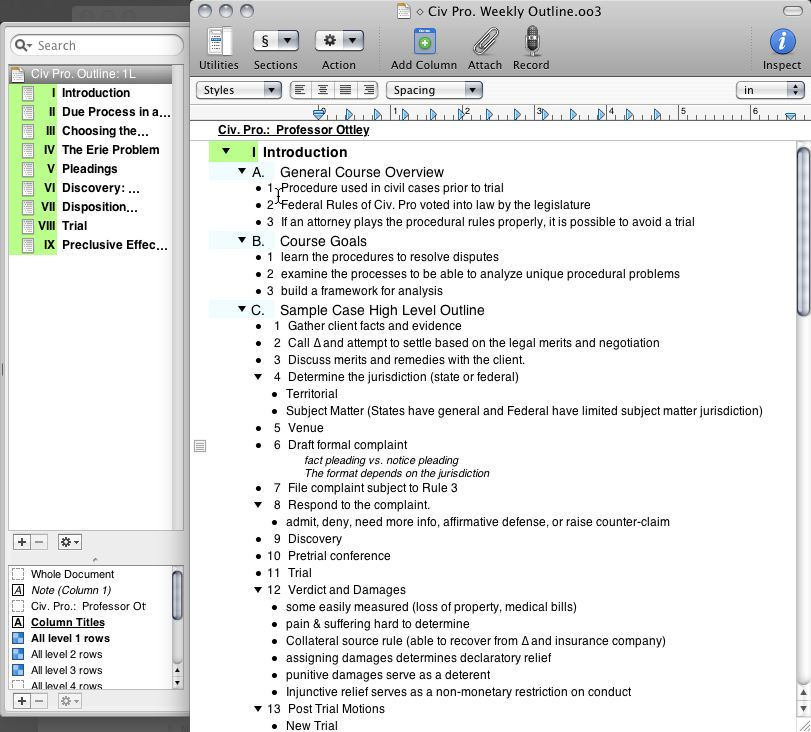
\includegraphics[width=\textwidth]{grafik/omnioutliner-screenshot} 
  \end{center}
  \caption{Screenshot of OmniOutliner \cite{omnioutliner:screenshot}}
  \label{fig:omnioutliner-screenshot} 
\end{figure}



\subsection{Gartner's hype cycle}
\label{subsec:hype-cycle}

The hype cycle highlights the phases of public attention that new technologies go through after their introduction. The X-axis symbolises the time after introduction, the Y-axis the intensity of attention for that technology.

\medskip
\begin{figure}[H] 
  \begin{center}
    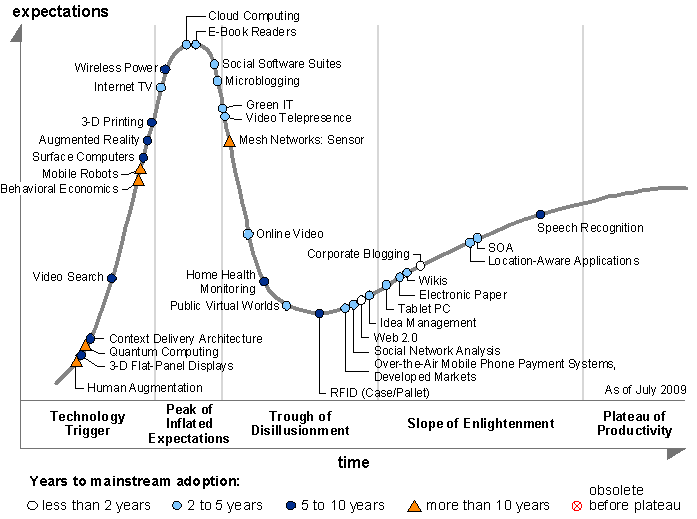
\includegraphics[width=\textwidth]{grafik/gartner-hype-cycle-2009} 
  \end{center}
  \caption{Gartner's 2009 hype cycle, \cite{cloud:hypecycle}}
\end{figure}


